\documentclass[lualatex]{beamer}
\usepackage[english]{babel}
\usepackage{graphicx}

\setbeameroption{show notes}
%\setbeameroption{hide notes}
\usetheme{Madrid}

\title[Kanban]{A Practical Introduction to Kanban}
  \author{Taoda}
  \institute{YITU tech}
  \date{July\ 2018}

\begin{document}

\begin{frame}
\titlepage
\end{frame}

\begin{frame}
  \frametitle{Outline}
  \tableofcontents
\end{frame}

\section{Flow}

\subsection{Flow}

\begin{frame}
  \frametitle{Flow}
  \begin{center}
    \Huge
    What is our dev flow?
  \end{center}
\end{frame}

\begin{frame}
  \frametitle{Flow}
  \begin{block}{Stages}
    \begin{itemize}
    \item Stages: where work items will stay for a while
    \item What is the exit?
      \note[item]{
        Exit:
        \begin{itemize}
        \item Is it Test Done? Is it Release?
        \item Theoretically speaking, the exit must bring some business value.
        \item It is okey to discuss a criterion per iteration.
        \end{itemize}
      }
    \item What is the entrance?
      \note[item]{
        Entrance:
        \begin{itemize}
        \item Generally speaking, Requirement is not a good entrance.
          Requirements are outputs from product designing.
          For teams with both PD and Dev, it is wise to involve product designing into iterations.
        \item Some ``requirements'' are not functional, or even not from PD.
          They are from Dev.
          For example, refactory.
        \item What about bug fixing?
          What about supporting?
        \item 
          my suggestion: the flow starts from Ideas.
        \end{itemize}
      }
    \end{itemize}
  \end{block}
\end{frame}

\begin{frame}
  \frametitle{Flow}

  \begin{block}{Queue}
    \begin{itemize}
    \item Queues are common blockers caused by limited bandwidth.
    \item So, it is wise to visualize them.
    \end{itemize}
  \end{block}
\end{frame}

\subsection{Lane}

\begin{frame}
  \frametitle{Flow}

  \begin{block}{Lane}
    \begin{itemize}
    \item Lanes: parallel activities
    \item One lane per project
      \begin{itemize}
      \item There are possibly many lanes, and most of them are empty.
      \end{itemize}
    \item One lane per person
      \begin{itemize}
      \item Work items may cross lanes.
      \item Where to place work items without owners? 
      \end{itemize}
    \item and, \dots
    \end{itemize}
  \end{block}
\end{frame}

\begin{frame}
  \frametitle{Flow}

  \begin{block}{Expedite Lane}
    \begin{itemize}
    \item a common way to handle urgent work items
    \end{itemize}
  \end{block}
\end{frame}

\subsection{WIP Limitation}

\begin{frame}
  \frametitle{WIP Limitation}

  \begin{block}{WIP Limitation}
    \begin{itemize}
    \item not rules, just triggers to discussions
    \item they are usually assigned on columns(stages), rows(lanes), and/or persons.
    \end{itemize}
  \end{block}
\end{frame}

\section{Work Item}

\begin{frame}
  \frametitle{Board and Work Items}
  \begin{center}
    \Huge
    Physical, or Electronic?
  \end{center}
  \note[item]{
    A physical board is always a good place where team members talk with each other.
    It is easy for outsiders to know what's happening about the team.
    But it is fragile.
    Stickies on it always fall down.
  }
  \note[item]{
    An electronic board is always available.
    It can track more things.
    It can be analyzed by programs.
    It even enables remote working.
  }
\end{frame}

\begin{frame}
  \frametitle{Work Items}
  \begin{center}
    \Large
    What must be there?
    \\
    What must be there on the 1st page?
  \end{center}
  \note[item]{
    For electronic ones, there usually are small squares delegated to work items.
    We can design what must be there on these small squares.
  }
\end{frame}

\begin{frame}
  \frametitle{Work Items}

  \begin{block}{Candidates}
    \begin{itemize}
    \item types of work: feature development, bug fixing, tech support, ...
    \item title
    \item avatar
    \item size of work item
    \item progress indicator
    \item urgency
    \end{itemize}
  \end{block}
\end{frame}

\section{Help The Work to Flow}

\begin{frame}
  \frametitle{Help The Work to Flow}

  \begin{block}{Daily standup}
    \begin{itemize}
    \item Kanban daily standup is also a short, timeboxed meeting, like those in Scrum.
    \item But it focuses on flows and solutions to make flows healthy.
      \begin{itemize}
      \item Are there anything hinder you from progressing?
      \item Are there smells on the board?
        \begin{itemize}
        \item broken WIP limitation
        \item hands on less urgent items
        \item too many items on a single hand
        \item items live too long
        \end{itemize}
      \end{itemize}
    \end{itemize}
  \end{block}
  \note[item]{
    By contrast, People in scrum standups talk:
    \begin{itemize}
    \item What did they do yesterday?
    \item What are they going to do today?
    \item Do they have any impediments that hinder them from doing that?
    \end{itemize}
  }
\end{frame}

\begin{frame}
  \frametitle{Help The Work to Flow}

  \begin{center}
    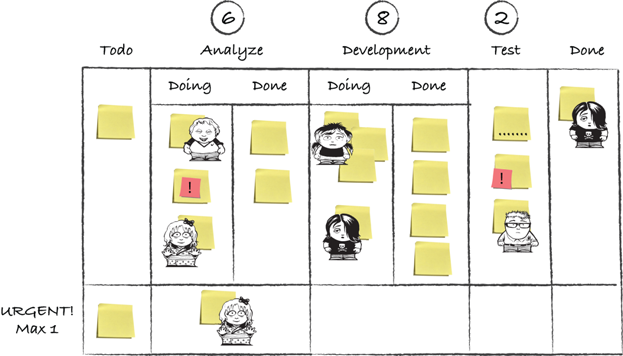
\includegraphics[width=\textwidth]{bad_smells.png}
  \end{center}
  \note[item]{
    Answer candidates are:
    \begin{itemize}
    \item No hands are on urgent items.
    \item An item takes too long to stay under Test.
    \item Too many items lays in the Urgent lane.
    \item Too many items stays under Development/Test.
    \item One hand is still on a Done item.
    \end{itemize}
  }
\end{frame}

\section{Philosophy}

\begin{frame}
  \frametitle{Philosophy: Focusing on Latency}
  \note[item]{
    By contrast, Scrum focuses on risk of releasing.
  }

  \begin{block}{Why Latency?}
    \begin{itemize}
    \item Latency itself brings business value.
      \note[item]{
        Most of teams do not touch latency-throughput margin.
        Those touching this line, I guess, do not really care of throughput.
      }
    \item Less latency means quick feedback, and quick feedback means less rework.
    \item Kanban provides tools (queues, WIP limitation) to \emph{visually} identify bottlenecks.
    \end{itemize}
  \end{block}
\end{frame}

\begin{frame}
  \frametitle{Philosophy: Evolving and Self-Organized}

  \begin{block}{Evolving, Self-Organized}
    \begin{itemize}
    \item Standups are for identifying bottlenecks, not for reporting progress.
    \item When bottlenecks are identified, the whole teams have to discuss a solution.
      \begin{itemize}
      \item the whole team designs workflow and work items.
      \item changing either workflow or work items is also a decision of the team.
      \end{itemize}
    \end{itemize}
  \end{block}
\end{frame}

\begin{frame}
  \frametitle{}
  \begin{center}
    \Huge
    Questions?
  \end{center}
\end{frame}

\end{document}
